\documentclass{sigchi}\usepackage[]{graphicx}\usepackage[]{color}
%% maxwidth is the original width if it is less than linewidth
%% otherwise use linewidth (to make sure the graphics do not exceed the margin)
\makeatletter
\def\maxwidth{ %
  \ifdim\Gin@nat@width>\linewidth
    \linewidth
  \else
    \Gin@nat@width
  \fi
}
\makeatother

\definecolor{fgcolor}{rgb}{0.345, 0.345, 0.345}
\newcommand{\hlnum}[1]{\textcolor[rgb]{0.686,0.059,0.569}{#1}}%
\newcommand{\hlstr}[1]{\textcolor[rgb]{0.192,0.494,0.8}{#1}}%
\newcommand{\hlcom}[1]{\textcolor[rgb]{0.678,0.584,0.686}{\textit{#1}}}%
\newcommand{\hlopt}[1]{\textcolor[rgb]{0,0,0}{#1}}%
\newcommand{\hlstd}[1]{\textcolor[rgb]{0.345,0.345,0.345}{#1}}%
\newcommand{\hlkwa}[1]{\textcolor[rgb]{0.161,0.373,0.58}{\textbf{#1}}}%
\newcommand{\hlkwb}[1]{\textcolor[rgb]{0.69,0.353,0.396}{#1}}%
\newcommand{\hlkwc}[1]{\textcolor[rgb]{0.333,0.667,0.333}{#1}}%
\newcommand{\hlkwd}[1]{\textcolor[rgb]{0.737,0.353,0.396}{\textbf{#1}}}%

\usepackage{framed}
\makeatletter
\newenvironment{kframe}{%
 \def\at@end@of@kframe{}%
 \ifinner\ifhmode%
  \def\at@end@of@kframe{\end{minipage}}%
  \begin{minipage}{\columnwidth}%
 \fi\fi%
 \def\FrameCommand##1{\hskip\@totalleftmargin \hskip-\fboxsep
 \colorbox{shadecolor}{##1}\hskip-\fboxsep
     % There is no \\@totalrightmargin, so:
     \hskip-\linewidth \hskip-\@totalleftmargin \hskip\columnwidth}%
 \MakeFramed {\advance\hsize-\width
   \@totalleftmargin\z@ \linewidth\hsize
   \@setminipage}}%
 {\par\unskip\endMakeFramed%
 \at@end@of@kframe}
\makeatother

\definecolor{shadecolor}{rgb}{.97, .97, .97}
\definecolor{messagecolor}{rgb}{0, 0, 0}
\definecolor{warningcolor}{rgb}{1, 0, 1}
\definecolor{errorcolor}{rgb}{1, 0, 0}
\newenvironment{knitrout}{}{} % an empty environment to be redefined in TeX

\usepackage{alltt}

\toappear{\scriptsize Permission to make digital or hard copies of all or part of this work for personal or classroom use is granted without fee provided that copies are not made or distributed for profit or commercial advantage and that copies bear this notice and the full citation on the first page. Copyrights for components of this work owned by others than ACM must be honored. Abstracting with credit is permitted. To copy otherwise, or republish, to post on servers or to redistribute to lists, requires prior specific permission and/or a fee. Request permissions from permissions@acm.org. \\
{\emph{L@S 2015}}, March 14--18, 2015, Vancouver, BC, Canada. \\
Copyright is held by the owner/author(s). Publication rights licensed to ACM. \\
ACM 978-1-4503-3411-2/15/03…\$15.00 \\
http://dx.doi.org/10.1145/2724660.2724680}

% Load basic packages
\usepackage{balance}  % to better equalize the last page
\usepackage{graphics} % for EPS, load graphicx instead
\usepackage{times}    % comment if you want LaTeX's default font
\usepackage{url}      % llt: nicely formatted URLs
\usepackage{booktabs}
\usepackage{rotating}


% llt: Define a global style for URLs, rather that the default one
\makeatletter
\def\url@leostyle{%
  \@ifundefined{selectfont}{\def\UrlFont{\sf}}{\def\UrlFont{\small\bf\ttfamily}}}
\makeatother
\urlstyle{leo}


% To make various LaTeX processors do the right thing with page size.
\def\pprw{8.5in}
\def\pprh{11in}
\special{papersize=\pprw,\pprh}
\setlength{\paperwidth}{\pprw}
\setlength{\paperheight}{\pprh}
\setlength{\pdfpagewidth}{\pprw}
\setlength{\pdfpageheight}{\pprh}

% Make sure hyperref comes last of your loaded packages, 
% to give it a fighting chance of not being over-written, 
% since its job is to redefine many LaTeX commands.
\usepackage[pdftex]{hyperref}
\hypersetup{
pdftitle={Attrition and Achievement Gaps in Online Learning},
pdfauthor={Rene F. Kizilcec, Sherif Halawa},
pdfkeywords={Online education; massive open online course; MOOC; persistence; dropout; individual differences; inequality; volition; social belonging; growth mindset; goal striving},
bookmarksnumbered,
pdfstartview={FitH},
colorlinks,
citecolor=black,
filecolor=black,
linkcolor=black,
urlcolor=black,
breaklinks=true,
}

% create a shortcut to typeset table headings
\newcommand\tabhead[1]{\small\textbf{#1}}

\clubpenalty=9996
\widowpenalty=8500


% End of preamble. Here it comes the document.
\IfFileExists{upquote.sty}{\usepackage{upquote}}{}
\begin{document}

\title{Attrition and Achievement Gaps in Online Learning}

\numberofauthors{2}
\author{
  \alignauthor Ren\'{e} F. Kizilcec\\
    \affaddr{Department of Communication}\\
    \affaddr{Stanford University}\\
    \email{kizilcec@stanford.edu}\\
  \alignauthor Sherif Halawa\\
    \affaddr{Department of Electrical Engineering}\\
    \affaddr{Stanford University}\\
    \email{halawa@stanford.edu}\\
}

\maketitle

\begin{abstract}
Attrition in online learning is generally higher than in traditional settings, especially in large-scale online learning environments. A systematic analysis of individual differences in attrition and grades in 20 massive open online courses ($N>67,000$) revealed a global achievement gap and a gender achievement gap. Online learners in Africa, Asia, and Latin America scored substantially lower grades and were up to half as likely to persist than those in Europe, Oceania, and Northern America. Women also exhibited lower persistence and performance then men. Yet more persistent learners were only marginally more satisfied with their achievement. The primary obstacle for most learners was finding time for the course, which was partly related to low levels of volitional control. Self-ascribed successful learners reported higher levels of goal striving, growth mindset, and feelings of social belonging than unsuccessful ones ($N=756$). 
Insights into why learners leave online courses informs models of attrition and targeted interventions to support learners achieve their goals.
\end{abstract}

\keywords{Online education; massive open online course; MOOC; persistence; dropout; individual differences; self-regulation; volition; social belonging; growth mindset; goal striving}

\category{K.3.1.}{Computers and Education}{Computer Uses in Education}
\category{H.5.m.}{Information Interfaces and Presentation (e.g. HCI)}{Miscellaneous}


\section{Introduction}

Educational environments have become increasingly diverse in format. Traditional schools and universities have a characteristically rigid structure, including instructor-defined syllabi, fixed time schedules, entry requirements, and material costs to enter and exit. Novel institutional structures have been developed to overcome particular constraints. Community colleges, for instance, were created in an attempt to democratize education by offering instruction at a lower cost, with lower admission criteria, and with more flexible schedules to accommodate those who cannot afford to be full-time students \cite{goldrick2010challenges}. Distance learning programs deliver education to remote parts of the world and to people who simply could not attend in-person classes. Course materials, including assessments, were delivered through mail (correspondence education), radio, television, and eventually the Internet, thereby addressing geographical and time related constraints of traditional instruction \cite{moore1996distance}.

The latest generation of online learning environments, characterized by massive open online courses (MOOCs), has pushed the boundary on the scale of education \cite{waldrop2013campus}. By design, MOOCs provide course materials to millions of people worldwide. This scale could be achieved by pre-recording lectures, designing assessments that can be graded automatically, and by leveraging the momentum of the number of people involved (e.g., to facilitate peer learning or peer assessment). Maybe by virtue of their large scale, their prominent instructors, or their adherence to contemporary interface designs, MOOCs rapidly became an online media phenomenon. People would sign up weeks in advance of the course launch date, many of whom would never even enter the course site. And among those who enroll and enter the site, a large proportion tends to only ``sample'' some content and leave again \cite{kizilcec2013deconstructing}. Many of the prototypical behaviors observed in MOOCs resemble those on online media platforms \cite{kizilcec2013deconstructing,breslow2013studying}. This trend is also reflected in the large spectrum of learners' motivations for enrolling in MOOCs \cite{kizilcec2015motivation}.

Shortly after the first wave of courses had finished, extensive media coverage led to MOOCs becoming associated with high attrition rates \cite{lewin2013after,parr2013mooc}. Early MOOC research cautioned against dichotomizing learners into successes and failures based on course completion \cite{kizilcec2013deconstructing,rivard2013measuring}. Instead, more nuanced categorizations based on learner behavior \cite{kizilcec2013deconstructing,clow2013moocs}, motivations \cite{kizilcec2015motivation}, or intentions \cite{wilkowski2014student} have been suggested. Perspectives on attrition in open online courses ultimately depend on how these courses are viewed. For instance, MOOCs can be thougth to have bridged two worlds: one is governed by the user-centric norms of online media, where everyone is encouraged to be as active as they wish; the other adheres to the ``grammar of schooling'' \cite{tyack1994grammar}, which presupposes instructor-defined goals that students strive to achieve \cite{kizilcec2015motivation}. This view of MOOC participation clearly adds complexity to interpretations of attrition. The present work extends the empirical base of research on attrition to inform the theoretical discourse and pave the path for novel practices.

This paper presents a systematic investigation of attrition in online learning based on self-report and behavioral data collected from over 100,000 learners in 21 courses in total. Identifying characteristics associated with attrition and reasons for disengaging can facilitate earlier recognition of learners struggeling to achieve their learning goals. These learners could benefit from changes to the course or targeted interventions. We briefly review the large literature on attrition in educational environments, with a focus on key developments in understanding the causes of attrition. Building on this review, Study 1 offers insights into reasons for disengaging from MOOCs, learners' satisfaction, and individual differences in attrition and performance. For Study 2, we invited around 6,053 learners who were predicted to have disengaged from a MOOC to provide feedback. We examined differences in psychological factors between subjectively successful and unsuccessful learners, and investigated the role of volitional control for those who reported having not enough time. Learners' open responses about challenges they faced while taking the course were iteratively coded to develop an empirically-grounded list of reasons for attrition.

\begin{table*}[th]
\caption{Summary statistics for 20 massive open online courses}
\small
\center
\label{tab:s1sum}
\begin{tabular}{llccccccccccc}
% & & & & & & & & $>$ 30\% & $>$ 50\% & $>$ 80\% & Self-Rep. \\
% & Topic Area & Enrollment & Course survey & Feedback survey & Female & Age & Education & videos & videos & videos & Dropout \\
\toprule
 &            &          & \multicolumn{3}{c}{Survey Responses} & & & & & \multicolumn{3}{c}{Videos Watched} \\
 \cmidrule(r){4-6} \cmidrule(r){11-13}
 & Topic Area & Enrolled & Initial & Feedback & Both & Female & Age$^1$   & Education$^2$ & Dropout$^3$ & $>$ 30\% & $>$ 50\% & $>$ 80\% \\
\midrule
C1 & Business & 61,233 & 8,618 & 1,796 & 1,282 & 47\% & 36 (28,43) & 94\% & 11\% & 11\% & 9\% & 6\%\\
C2 & Business & 45,202 & 5,951 & 789 & 631 & 43\% & 36 (27,42) & 90\% & 10\% & 11\% & 8\% & 6\%\\
C3 & Computer Science & 28,086 & 5,918 & 2,815 & 2,295 & 36\% & 33 (23,40) & 63\% & 3\% & 15\% & 11\% & 8\%\\
C4 & Computer Science & 56,314 & 2,686 & 749 & 352 & 14\% & 33 (25,39) & 79\% & 21\% & 13\% & 10\% & 8\%\\
C5 & Computer Science & 79,273 & 7,319 & 1,740 & 1,236 & 16\% & 31 (24,36) & 81\% & 11\% & 15\% & 11\% & 8\%\\
C6 & Education & 40,214 & 24,192 & 5,174 & 4,969 & 56\% & 28 (15,40) & n.a. & 5\% & 17\% & 13\% & 8\%\\
C7 & Education & 5,325 & 2,429 & 624 & 615 & 80\% & 43 (35,50) & 99\% & 2\% & 24\% & 17\% & 12\%\\
C8 & Engineering & 11,958 & 2,341 & 262 & 196 & 16\% & 35 (26,43) & 84\% & 16\% & 14\% & 9\% & 6\%\\
C9 & Engineering & 5,701 & 5,652 & 396 & 347 & 16\% & 33 (24,38) & 73\% & 16\% & 18\% & 11\% & 7\%\\
C10 & Engineering & 7,139 & 1,250 & 197 & 168 & 17\% & 31 (22,36) & 72\% & 7\% & 11\% & 8\% & 6\%\\
C11 & Humanities & 7,656 & 2,512 & 142 & 131 & 89\% & 33 (24,38) & 82\% & 9\% & 14\% & 9\% & 6\%\\
C12 & Humanities & 4,949 & 2,921 & 292 & 270 & 91\% & 33 (25,38) & 83\% & 17\% & 15\% & 10\% & 7\%\\
C13 & Mathematics & 49,509 & 3,031 & 836 & 510 & 35\% & 37 (26,47) & 76\% & 32\% & 12\% & 9\% & 6\%\\
C14 & Mathematics & 13,310 & 2,861 & 346 & 298 & 10\% & 31 (25,34) & 93\% & 15\% & 15\% & 10\% & 6\%\\
C15 & Natural Sciences & 9,918 & 3,957 & 1,351 & 1,223 & 51\% & 37 (26,47) & 78\% & 4\% & 19\% & 15\% & 11\%\\
C16 & Natural Sciences & 543 & 163 & 79 & 50 & 47\% & 34 (26,39) & 98\% & 18\% & 27\% & 20\% & 12\%\\
C17 & Physics & 6,452 & 1,069 & 269 & 269 & 14\% & 36 (25,46) & 82\% & 11\% & 15\% & 10\% & 6\%\\
C18 & Statistics & 11,733 & 11,465 & 1,837 & 1,569 & 22\% & 36 (28,41) & 96\% & 9\% & 34\% & 25\% & 15\%\\
C19 & Statistics & 13,161 & 3,495 & 819 & 627 & n.a. & n.a. & n.a. & 6\% & 13\% & 9\% & 7\%\\
C20 & Writing & 35,374 & 12,514 & 2,877 & 2,876 & n.a. & n.a. & n.a. & 8\% & 23\% & 14\% & 8\%\\
\bottomrule
\multicolumn{13}{l}{$^1$ mean (upper, lower quartile)  $^2$ bachelor's or higher degree  $^3$ self-reported in the feedback survey}
\end{tabular}
\end{table*}


\section{Related Work}

Research and theory on attrition has a rich history in education. This review focuses on how conceptions of attrition have evolved over the last decades.  As this review is intended to serve as a foundation to build on with the current research, we concurrently develop hypotheses and research questions to investigate.

\subsection{In-person Education}

The majority of early work on attrition centered around theoretical models of students' decision to persist or dropout of a traditional higher education setting. The literature on attrition in higher education is largely concerned with students disengaging from a course of study rather than a single course. An early model suggested that students' presistence is largely driven by their prior behavior, attitudes, and norms \cite{fishbein1975belief}. The psychological processes involved in turning an intent to learn into the decision to persist were thought to be mediated by volition, the extent to which the student engages in goal-directed behavior in the face of distraction \cite{corno1993role}. Motivation alone is necessary but not sufficient for persistence, because students may fail to sustain efforts in the absence of strong self-regulatory skills.

\begin{description}
  \item[H1] Successful learners exhibit higher levels of goal striving than unsuccessful learners.
\end{description}

The next generation of psychological models, which were highly influential in the literature, emphasized the critical role of students' ``fit'' in the institution. Tinto's \citeyear{tinto1975dropout} student integration model posited that college students' decision to persist is a function of prior experiences and individual students' characteristics, and experiences during college. While prior experiences and characteristics are fixed, schools can influence the college experience, including the degree of social and academic integration. Tinto operationalized academic and social integration by GPA scores and the frequency of positive interactions with peers and instructors, respectively. This resonates with recent work highlighting the critical role of students' feelings of social belonging in achievement-oriented environments (e.g. \cite{walton2007question}). 

\begin{description}
  \item[RQ1] How are prior characteristics (demographics, geographic location, intentions, and prior experience) related to learners' likelihood of disengaging from the course?
  \item[H2] Successful learners exhibit a greater sense of social belonging than unsuccessful learners.
\end{description}

Tinto's work, which specifically targets traditional college students, prompted universities to be proactive in establishing environments that support student integration. Research on attrition in community college settings reiterates the importance of academic and social integration, but points out that non-persistence could indicate success depending on students' intent---students may leave after accomplishing their goal \cite{bers1991persistence}. Nevertheless, a brief psychological intervention that taught community college students an incremental theory of intelligence (instilling a growth mindset \cite{dweck2006mindset}) was found to halve attrition rates and increase academic achievement \cite{paunesku2012brief}. This highlights the critical role of mindset and caution against overinterpreting non-persistence as an indicator of goal achievement.

\begin{description}
  \item[RQ2a] What proportion of learners who disengaged were satisfied with their achievements in the course?
  \item[RQ2b] How does learners' level of satisfaction depend on their behavior in the course?
  \item[H3] Successful learners have a more growth mindset than unsuccessful learners.
\end{description}

\subsection{Distance Education and e-Learning}

Distance education, relative to traditional in-person education, tends to attract a more mature student demographic and provide fewer opportunities for social integration. Students in distance learning programs are more likely to lead social lives outside of school, maybe working part-time and living with their partner. Building on Tinto's model, Bean and Metzner \citeyear{bean1985conceptual} proposed a conceptual model of persistence that would be more applicable to nontraditional students. Persistence is thought to be a function of background characteristics (demographics, etc.), academic and environmental variables (study habits, financial resources, work and family obligations, etc.), and academic and psychological outcomes (GPA, satisfaction, etc.). The significant change from Tinto's orginal model was the inclusion of environmental variables to account for the added complexity of nontraditional students' lives.
% (see \cite{kember1989longitudinal}, for another adaptation of Tinto's model for distance education).

Rovai \citeyear{rovai2003search}, combining Tinto's and Bean and Metzner's models with factors specific to online learning and pedagogical styles, proposed a composite persistence model specifically for students in online distance education programs. Among other novel factors, Rovai's model acknowledges the critical role of computer literacy in online learning. And yet, these increasingly complex theoretical models were difficult to apply to real-world settings, and hence, the empirical evidence to support them remained sparse. An exploratory study of reasons for attrition of over 1,000 online students found eight relevant factors: academic and technical skills, learner motivation, time and support for studies, cost and access to the Internet, and technical problems \cite{muilenburg2005student}. An analysis of student behavior on an online education platform showed that 31\% of variation in achievement could be accounted for by a small set of participation measures \cite{morris2005tracking}.

\subsection{MOOCs}

A survey of over a hundred learners who dropped out of a MOOC showed that the majority indicated having too little time due to work responsibilities, not enough social support inside and outside of the course, and insufficient academic and technical support from the course \cite{gutl2014attrition}. A qualitative analysis of public records, especially forum posts, from 42 MOOCs suggested the following reasons for attrition: lack of time, learner motivation, feelings of isolation, lack of interactivity, insufficient prior knowledge or skills, and hidden costs \cite{khalil2014moocs}. A survival analysis of close to 800 learners who had posted on a MOOC discussion forum suggested that the likelihood of dropout was lower for those who i. actively participated in the first week of the course; ii. served as an authority figure in the community on the forum, and iii. did not engage in a particular subcommunity on the forum \cite{yang2013turn}. In addition, a number of machine learning approaches yielded promising results for early dropout prediction (e.g. \cite{taylor2014likely,halawa2014dropout}), but fell short of offering insights into why a given learner would leave the course.

\begin{description}
\item[RQ3a] What reasons do learners report for disengaging from a course?
\item[RQ3b] How do reasons for disengaging vary by learner characteristics?
\end{description}  

\begin{knitrout}
\definecolor{shadecolor}{rgb}{0.969, 0.969, 0.969}\color{fgcolor}\begin{figure*}[ht]

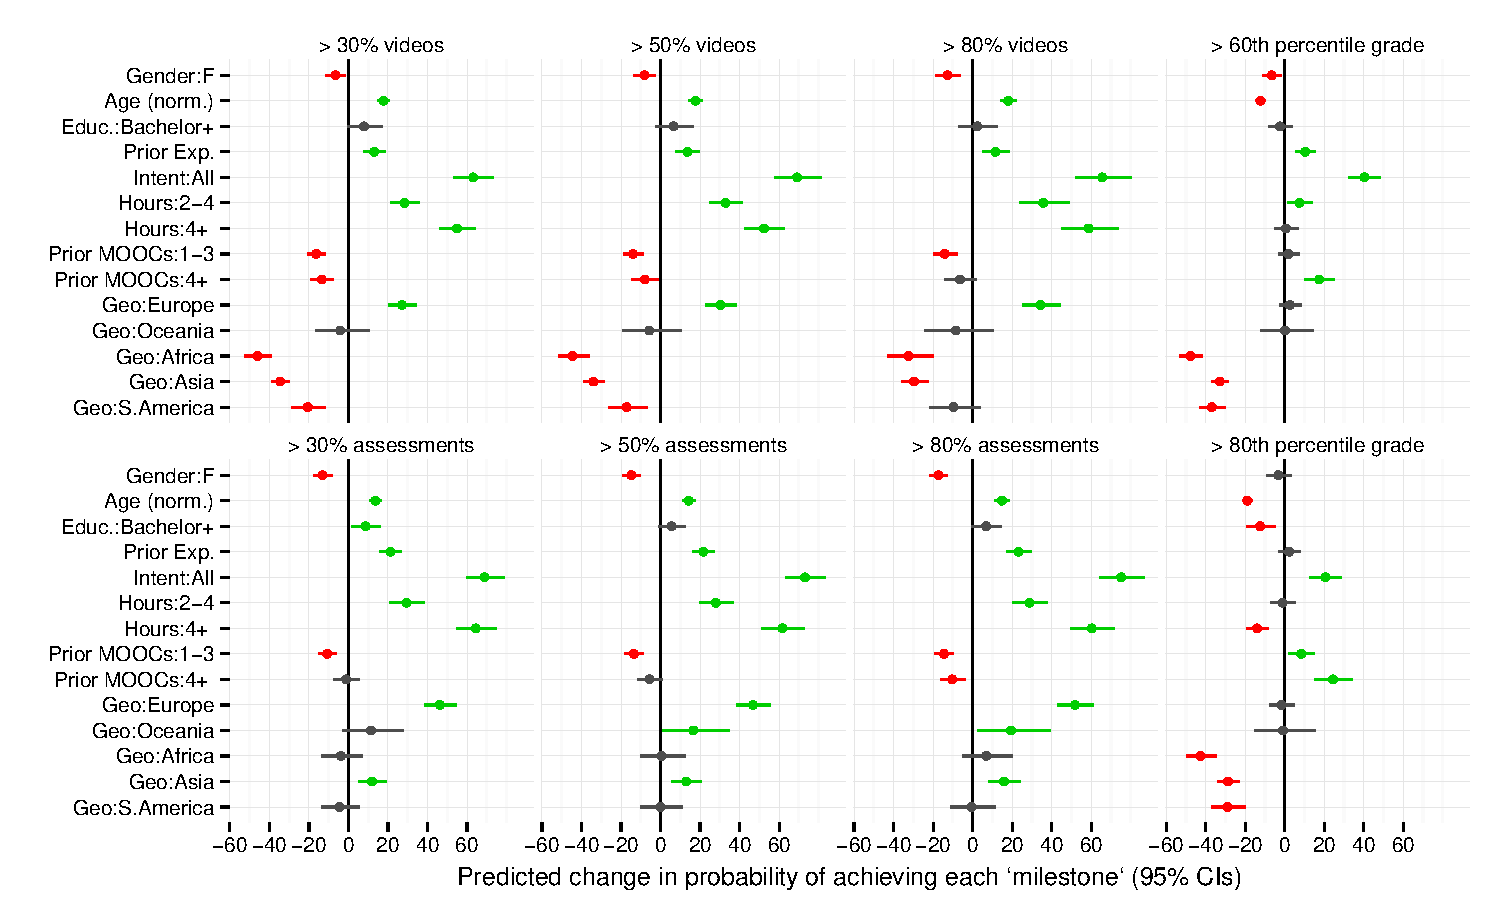
\includegraphics[width=\maxwidth]{figure/s1coefs} \caption[Individual differnces in persistence and course grades showing substantial achievement gaps]{Individual differnces in persistence and course grades showing substantial achievement gaps. An estimate of -10 indicates a 10\% lower chance of achieving a milestone.\label{fig:s1coefs}}
\end{figure*}


\end{knitrout}

\section{Study 1: Attrition \& Satisfaction}

The present study extends the existing literature on attrition with a large-scale quantitative treatment of attrition in MOOCs. We address the research questions developed in the previous section with the larger objective of informing our understanding of attrition in online courses to better support learners. This could be achieved through general changes to the course content or presentation; or, using targeted interventions that support particular groups of struggeling learners.

\subsection{Methods}

Twenty MOOCs on topics in a variety of disciplines were selected for investigation. Table \ref{tab:s1sum} provides summary statistics for enrollment, survey response rates, demographics, self-reported dropout, and a subset of behavioral indicators for each course. For each course, we combined data from an initial course survey (distributed in the first weeks of the course), a feedback survey (distributed in the last weeks of the course), and behavioral data collected in the learning environment. On the initial course survey, learners reported their gender, age, education, prior experience with the topic and MOOCs, and how many hours per week they intend to spend on the course. On the feedback survey, learners reported their satisfaction with the course (5-item index, possible range from 0 to 5.2, $M=3.95, SD=0.81, \alpha=.81$), and whether they `stopped participating in the course before it ended' or `remained active until the end'. Those who indicated that they stopped participating also reported `what influenced their decision to stop participating' using a grid of 14 binary-choice items (cf. Figure \ref{fig:s1reason}).\footnote{Instead of a select-all-that-apply question, this question style encouraged learners to consider each reason separately. The response options were ``Did influence my decision to stop" and ``Did NOT influence my decision to stop" to reduce acquiescence bias relative to a Yes/No or Agree/Disagree scale.} Geographic location was determined by IP address and aggregated by continental region. Behavioral indicators were chosen to represent course milestones: watching (or downloading) over 30\%, 50\%, 80\% of lecture videos, attempting over 30\%, 50\%, 80\% of assessments, and achieving a grade above the 60$^\text{th}$, 80$^\text{th}$ percentile. 

To analyze individual differences, we fit a logistic mixed-effects (hierarchical) model predicting binary persistence and performance milestones using learner characteristics, including demographic and geographic features. The analysis included 67,333 learners who completed the initial course survey, but excluded 381 learners who left all questions unanswered and learners in courses C6, C7, C19, C20 due to missing survey items. Any remaining missing survey responses were multiply imputed using other survey responses. We report pooled estimates that account for added uncertainty.\footnote{Multiple imputation ($m=10$) using the $R$ mice package.} Correlations between predictors were low ($|r|<0.15$), except for age and education ($r=0.27$), which were each significant predictors if the other was excluded. Courses were modeled as a random effect (instead of including dummy variables) to generalize to a larger population of similar MOOCs.




\subsection{Results and Discussion}

We address the posed research questions in three parts: first, a regression analysis of differential attrition and performance ($RQ1$); second, a comparison of satisfaction levels across learner subgroups ($RQ2$), and third, a descriptive analysis of reported reasons for disengaging from the course ($RQ3$).

\subsubsection{Individual Differences in Attrition and Performance}

Individual differences in attrition and performance are illustrated in Figure \ref{fig:s1coefs} as transformed regression coefficients with 95\% confidence intervals for each milestone. The estimates represent changes in the likelihood of achieving a milestone relative to an arbitrary baseline population. The regression intercept corresponds to the following baseline group that derives from the coding of regressors: average-aged male learners in Northern America\footnote{Learners in the United States, Canada, Bermuda, Greenland.} without a bachelor's degree, without prior experience with the topic or other MOOCs, prepared to spend up to 2 hours/week on the course, and not intending to complete it. This choice notably corresponds to the dominant power structure narrative, but is solely statistically motivated. The baseline probability for each milestone was as follows: lectures watched (20\% above 30\%, 11\% above 50\%, 4\% above 80\%), assessments attempted (37\% above 30\%, 25\% above 50\%, 18\% above 80\%), and grades (30\% above the 60$^\text{th}$, 22\% above the 80$^\text{th}$ percentile).

A number of significant and substantial individual differences emerged. Women were 12 to 20\% less likely than men to persist with lectures and assessments. Women, who constituted 34\% of learners in the sample, were also 10\% (7\%) less likely than men to score a grade above the 60$^\text{th}$ (80$^\text{th}$) percentile.  Moreover, learners in Africa ($N = 2,458$), Asia ($N = 13,280$), and Latin America ($N = 5,344$) were 24 to 50\% less likely to persist with lectures and 31 to 52\% less likely to achieve grade milestones than learners in Northern America ($N = 26,651$). In contrast, learners in Europe ($N = 17,988$) exhibited 16 to 30\% higher persistence with lectures and assessemnts than learners in Northern America. While learners in Asia exhibited lower persistence with videos, they were at least as likely to attempt assessments as learners in North America. Learners in Oceania ($N = 1,612$) performed similarly to those in Northern America and Europe. Besides gender and geography, older learner were more likely to persist with lectures and assessments, but achieved lower grades than younger learners. More educated learners, those with a bachelor's or higher degree, were 15 to 25\% more likely to persist and 10\% more likely to score above the 60$^\text{th}$ percentile. Not surprisingly, prior experience, intending to learn about all topics in the course, and being prepared to spend more hours in the course were strong predictors of persistance. Learners who participated in prior MOOCs had mixed persistence patterns, but achieved higher grades.

The large scale of MOOCs has revealed a global achievement gap and a gender achievement gap in online learning. Performance and persistence in the course was substantially lower for women and learners in Africa, Asia, and Latin America than men and learners in Europe, Oceania, and Northern America. There was a good representation from each geographic region in the dataset and the courses under consideration were on diverse topics, including some in the humanities and business with high female participation rates. The strength and significance of these relationships is remarkable, in particular with several additional demographic, geographic, and preference measures in the model. The first generation of large-scale online learning, characterized by MOOCs, is apparently not immune to inequalities that have pervaded traditional educational settings. The present work presents evidence for the existence of these gaps, but cannot explain why they occur. Of course there exists no innate feature of women or people in certain locations that is responsible for these gaps. The achievement gaps could plausibly result from differences in Internet access, language barriers, or from feelings of psychological threat, such as fears of confirming a negative stereotype \cite{spencer1999stereotype} or not belonging in the course \cite{walton2007question}. A geographical categorization to compare countries with a high and low propensity of English speakers could be misleading, due to confounding with psychological barriers that are less likely to hinder learners in English-speaking countries. More work is needed to identify potential causal mechanisms underlying these gaps.

\begin{knitrout}
\definecolor{shadecolor}{rgb}{0.969, 0.969, 0.969}\color{fgcolor}\begin{figure*}[ht]

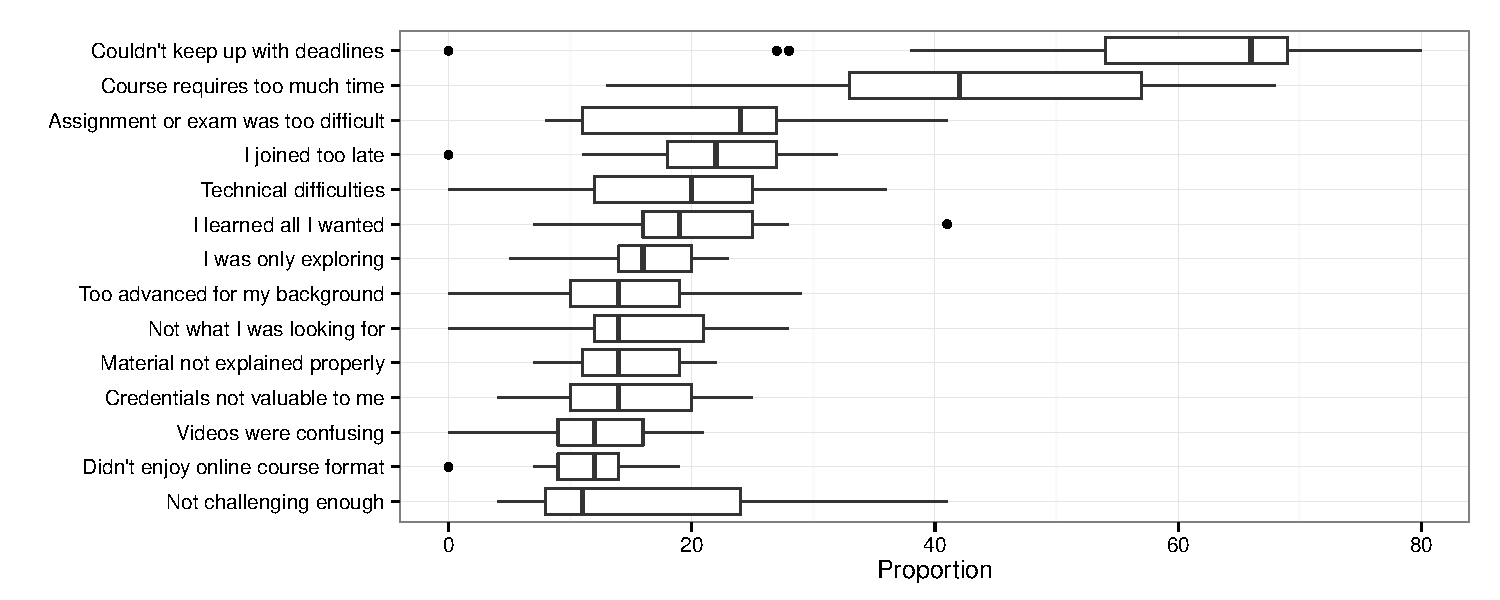
\includegraphics[width=\maxwidth]{figure/s1reason} \caption[Distribution of self-reported reasons for attrition across 20 MOOCs]{Distribution of self-reported reasons for attrition across 20 MOOCs.\label{fig:s1reason}}
\end{figure*}


\end{knitrout}

\subsubsection{Satisfaction}
% RQ2a: What proportion of learners who disengaged were satisfied with their achievements in the course?
% RQ2b: How does learners' behavior in the MOOC vary by their level of satisfaction?

Attrition can be a sign of success if a learner has achieved their personal learning objectives. We investigated how satisfied learners were with their achievements for those who reported to have stopped participating ($RQ2a$) and those who persisted to different extents ($RQ2b$). Satisfaction ratings were compared using mixed-effects regression ($N=23,390$). Learners who reported that they stopped participating were 12\% less satisfied than those who reported not to have stopped ($t_{453}=21, p<.001$). Moreover, we examined if persistent learners, those who watched more lectures, were also more satisfied. The proportion of videos significantly predicted higher satisfaction ($t_{101}=20, p<.001$), such that those who watched over 75\% of videos were 8\% more satisfied than those who watched under 25\% ($M_{<\text{25\%}}=3.80, M_{>\text{75\%}}=4.09$). As levels of self-reported satisfaction were generally high, it remains unclear if the estimated differences in satisfaction are consequential. Learners who disengaged early were only somewhat less satisfied than those who persisted in the course, which suggests that some learners arrived with modest course goals and achieved them. The following analysis of reasons for attrition can shed more light on this hypothesis.

\subsubsection{Reasons for Attrition}
% RQ3a: What reasons do learners report for disengaging from a MOOC?
% RQ3b: How do reasons for disengaging vary across prior learner characteristics (cf. RQ1)?

A fraction of learners who completed the course feedback survey reported having left the course early and indicated reasons for disengaging on a pre-defined list ($RQ3a$). This list may not be collectively exhaustive, which is addressed in Study 2, but responses were collected from 1,698 learners in 20 different courses. Figure \ref{fig:s1reason} illustrates how frequently each reason was selected across courses. Around half of the respondents indicated two time-related reasons as influencing their decision to stop participating. In a typical course (median proportion), 66\% faced issues keeping up with deadlines and for 46\% the course demanded too much time. According to expectancy-value theory, the learner is a rational agent who allocates time to different activities to maximize subjective gains. The shortage of time could be due to an abundance of higher-priority tasks, as enrolling in a MOOC neither guarantees that a learner can nor intends to allocate enough time to complete the course. Alternatively, a low capacity for volitional control \cite{corno2001volitional} could lead learners to misallocate time to lower-priority activities that promise nearer gratification, instead of allocating it to the next highest priority task. Learners' general time issues may be a product of high-priority obligations as well as a result of a low capacity for volitional control. We investigate this hypothesis in Study 2.

Other reasons for attrition were less prevalent, but still reported by around 10 to 25\% of respondents. Notably, 17\% of respondents in a typical course stopped participating because they learned all they intended to learn. This finding resonates with some prior work on attrition in community colleges, where attrition has been interpreted as a sign of success. It also supports the observation that progress in the course and satisfaction were only weakly related. We investigated the underlying factor structure of the reported reasons for disengaging using an exploratory factor analysis. The optimal number of factors was determined by the parallel analysis criterion and corresponding scree plot. The following four-factor solution emerged: first, {\em general time issues} (course requires too much time; can't keep up with deadlines);  second, {\em difficulty} (too advanced, exam too difficult); third, {\em format \& content} (didn't enjoy online format, confusing videos, materials not explained well, not what I'm looking for, technical difficulties), and fourth, {\em goals \& expectations} (only exploring, learned all I wanted, not challenging, credential not valuable). The `late start' item failed to load onto any factor. General time issues and difficulty are very interpretable factors, while the other two factors comprise a complex set of reasons that should probably be further separated.

Reasons for disengaging from a course are likely to vary by learner characteristics ($RQ3b$). To explore if the substantial individual differences in attrition identified above could be associated with different reasons for disengaging, we investigated variation by geographic region ($N = 1,698$) and gender ($N = 1,039$ due to missing gender information). Learners in Africa, Asia, and Latin America were more likely to disengage due to technical difficulties (61\% more likely), too demanding deadlines, and starting late ($p\text{s} < .03$), while learners in Europe, Oceania, and Northern America were more likely to disengage because the course was not a good fit for them ($p=.02$). Women were more likely than men to report disengaging due to technical difficulties and because the course required too much time ($p<.01$). Technical difficulties were a critical individual difference that could be a source of the observed achievement gaps. The pre-defined list of reasons for attrition unfortunately did not include an item on language difficulties, which could be another plausible source of the global achievement gap.


\section{Study 2: Understanding Attrition}

To gain a better understanding of the attrition patterns identified in Study 1, we designed a smaller, more focused follow-up study. This study investigates reasons for attrition based on psychological measures and learners' own descriptions of the challenges they faced. We collected feedback from learners who were likely to have stopped following the course. They were identified with a predictive model and invited to complete a survey. The survey included self-report measures of psychological constructs to test hypotheses $H1, H2,$ and $H3$ on the role of goal striving, social belonging, and growth mindset in the success of online learners. Moreover, in Study 1, most learners indicated that they disengaged due to a shortage of time. A variety of factors could influence the amount of time learners have at their disposal. Higher priority obligations, such as professional, academic, and personal committments are presumably large contributors. Another critical factor, especially in the context of MOOCs as largely unguided learning environments, is a learner's volitional control to engage in self-regulated learning \cite{corno2001volitional}. Low volitional control could reduce learners' ability to allocate time for the course in the presence of potential distractors of subjectively lower importance than taking the course (watching TV, etc.). In contrast to attrition due to important obligations, there exist techniques to help learners become more self-regulated, which could boost their persistence. We constructed the following hypotheses about the role of volition in time-related attrition:

\begin{description}
  \item[H4a] Learners who report having `not enough time' can be grouped into those with higher priority obligations (professional, academic, and personal) and those with low volitional control.
  \item[H4b] Learners who do not report specific higher-priority obligations tend to exhibit lower volitional control than those who specify particular obligations.
\end{description}  

\subsection{Methods}

The particular MOOC under observation was an undergraduate-level course on an advanced topic in computer science. It was offered in 2014 through Coursera. There were 20,048 enrolled learners; 10,510 watched at least one video, and 5,912 attempted at least one assignment. The following subsections describe how disengaging learners were identified, which measures were included in the feedback survey, and how open responses were iteratively coded.

\subsubsection{Predicting Disengagement}

We constructed an `early warning' prediction model to flag learners who had disengaged from the course or were about to disengage. The following three criteria were chosen as benchmarks to evaluate the practical and theoretical value of our prediction model.%   In order for our predictions to be useful, we need to observe the following three features of the dropout prediction problem.

\textit{Prediction accuracy}: Prediction recall (fraction of correctly predicted disengaged learners) should be high to deliver the survey to as many disengaged learners as possible. The false positive rate (fraction of active learners who are incorrectly predicted as disengaged) should be low to avoid sending surveys to learners who do not experience challenges in the course.

\textit{Prediction lag}: The period between a learner's last site activity and the time they are flagged as disengaged should be short. A shorter prediction lag improves the likelihood of successfully intervening to help learners resume the course.

\textit{Transferability}: Whether or not a learner disengages from the course cannot be determined before the end of the course. We thus trained the prediction model using data from previous courses. The performance of the prediction model should be good in courses other than those on which it was trained.

The training set was composed of learners' interaction data (predictors) and disengagement states (outcome) from 20 MOOCs. The large number of courses should improve model transferability by favoring features that are strongly predictive across different courses. Five hundred learners from each MOOC were included in the training set ($train$), and 500 other learners from the same MOOCs were selected for the first test set ($test_1$). A second test set of similar size was composed from 20 other MOOCs ($test_2$). Features extracted from the interaction data included different aspects of learners' video, assignment, and forum activity; their pace of viewing videos relative to the course pace, as well as various aspects of engagement time, such as the last time the learner interacted with the course (cf. \cite{halawa2014dropout}, for additional information on the prediction model).

To control the length of the prediction lag, the model was only provided with learners' activity data until they were absent for 14 consecutive days. In the training phase, if the learner disengaged but the model did not detect it within 14 days of their last activity, the case was counted as a false negative. This construction results in a model with features that all fall within the defined prediction lag period. The model was fit by logistic regression with two-fold learner-level and course-level cross-validation. Prediction performance measured by the area under the ROC curve (AUC) very high (0.931 for $train$, 0.929 for $test_1$, 0.922 for $test_2$). Two of the predictors in the fitted model are highly influential. The first is the number of days since the learner has last been active. The likelihood that the learner drops out increases substantially if the learner disengages for 14 days or more. However, the likelihood of such a learner re-engaging increases with the fraction of released videos the learner has viewed prior to the absence; this is the second most influential feature in the model. The fact that almost identical results were obtained for $test_1$ and $test_2$ suggest good transferability of the model. A learner was flagged if their dropout probability exceeded 50\%. Out of the 20,048 enrolled learners in the course, only those 10,510 were considered who watched at least one lecture video, and 6,074 of them were flagged as likely to drop out. The survey was sent out to 6,053 learners (excluding 21 learners with invalid email addresses or duplicate accounts).

\begin{table*}[ht]
\caption{Descriptive and inferrential statistics for psychological measures by self-ascribed success}
\label{tab:psych}
\center
\begin{tabular}{lcccc}
\toprule
 & $N$ & Goal Striving ($H1$) & Social Belonging ($H2$) & Growth Mindset ($H3$) \\
\midrule
\emph{Relative Progress} &  &  &  \\
\quad Successful & 241 & 3.46 $(SD=0.91)$ & 4.70 $(SD=0.74)$ &  4.58 $(SD=0.99)$ \\
\quad Unsuccessful & 515 & 2.96 $(SD=0.93)$ & 4.63 $(SD=0.70)$ & 4.38 $(SD=0.87)$ \\
 &  & $t_{201}=6.3, p<.001, d=0.55$ & $t_{60}=1.0, p>.25, d=.09$ & $t_{152}=2.4, p=.017, d=0.21$ \\
 \emph{Satisfaction} &  &  &  \\
\quad Successful & 325 & 3.43 $(SD=0.83)$ & 4.76 $(SD=0.70)$ & 4.47 $(SD=0.93)$ \\
\quad Unsuccessful & 431 & 2.88 $(SD=0.97)$ & 4.58 $(SD=0.71)$ & 4.42 $(SD=0.91)$ \\
&  & $t_{166}=7.2, p<.001, d=0.59$ & $t_{158}=3.1, p=.002, d=.26$ & $t_{175}=0.6, p>.25, d=.05$ \\
\bottomrule
\end{tabular}
\end{table*}

\subsubsection{Feedback Survey}

Every learner who was predicted to disengage from the course was sent an email kindly requesting their help: ``You are enrolled in [course name], but you've been less active recently. Could you help us understand why?'' A low response rate was expected for this subpopulation that was defined by low engagement. And yet, 756 out of 6,053 learners started the survey (12.5\% response rate), and 459 completed it (61\% completion rate). Missing values were multiply imputated by predictive mean matching using responses to all survey questions. All estimates were pooled across ten imputations, with standard errors adjusted for added variance. The majority of respondents were male (85\%), 35.6 years old on average ($SD=12.5$), and 80\% had achieved a bachelor's or more advanced degree.

Learners were asked to report how satisfied they were with their progress in the course, and whether they were using the course materials more, less, or exactly as much as they would have liked. These items served as measures of personal success. They were then asked to openly report ``what challenges, inside or outside of the course, [they] experienced while [they were] taking this course, if any?'' The instructions encouraged them to list all challenges they could think of. This question was asked prior to any survey questions that could suggest particular reasons for disengaging.

Two research assistants independently developed codebooks for the resulting 448 non-empty open responses. Their codebooks were consolidated and applied on Amazon Mechanical Turk (AMT) in three iterations. The codebook was updated in each iteration to reliably fit the open response data. Specific updates to the initial codebook were informed by code frequency, code correlations, and inter-coder agreement. In the first iteration, 250 randomly selected responses were each coded by four `classification experts,' which is an AMT-specific qualification. In the second iteration, the remaining responses were coded in the same way. In the final iteration, all responses were coded by two classification experts (ties were resolved by two researchers).\footnote{For additional details on the coding procedure and codebooks, see http://kizilcec.com/rsc/las2015attrition.pdf.} The iterative coding yielded 399 relevant coded responses, which were analyzed in combination with the remaining survey data.

Learners self-reported social belonging (17 items on their sense of social and academic fit \cite{walton2007question}, $M=4.66, SD=0.71, \alpha=0.86$); mindset (4 items on the stability of intelligence and talent\footnote{Adapted from http://mindsetonline.com/testyourmindset}; $M=4.44, SD=0.92, \alpha=0.77$), goal striving (4 items on motivation, perceived importance, committment, and confidence; $M=3.12, SD=0.95, \alpha=0.82$), and capacity for volitional control (one item on the extent to which lower-priority distractions have hindered the learner's course progress; $M=2.73, SD=1.29$).

\subsection{Results and Discussion}

We further investigated research question $RQ3a$ about reasons for disengaging from the course, and tested hypotheses $H4ab$ about volitional control. In a second set of analyses, we tested our hypotheses about the role of psychological factors in the self-ascribed success of MOOC learners.
\\
\subsubsection{Psychological Factors}

Hypotheses $H1$, $H2$, and $H3$ about goal striving, perceived social belonging, and mindset, respectively, were tested by comparing self-ascribed successful with unsuccessful learners. Self-ascribed success was measured by relative progress and satisfaction with progress: 68\% of respondents reported using the course materials less than they would have wanted, and 57\% reported not being satisfied with their progress in the course (18\% were very or extremely dissatisfied). The two measures of success were correlated, $r=.35, t_{754}=10, p<.001$; satisfied respondents were, however, equally likely to be successful and unsuccessful in terms of their progress. Table \ref{tab:psych} provides summary statistics for each psychological measure by these two success metrics. Successful learners exhibited higher levels of goal striving according to both progress and satisfaction measures. Social belonging was significantly higher for learners who were successful in terms of satisfaction, but not those who were successful in terms of progress. The pattern was reversed for growth mindset, such that learners who were successful in terms of progress (but not satisfaction) exhibited a stronger growth mindset. This pattern could reflect a difference in the underlying process by which these psychological factors affect learner behavior and perception. The observed differences are expected to be larger in the full population of learners, compared to the homogenous sample in this study, consisting of learners who most likely left the course.

Personal success in a MOOC was associated with three established psychological factors: goal striving, social belonging, and growth mindset. Prior work in more traditional achievement-oriented environments found reduced levels of these psychological factors to result in lower persistence and performance. The current observational findings highlight the critical role of these factors in an online learning environment. Learners with higher levels of goal striving, social belonging, and growth mindset reported greater personal success ($H1,H2,H3$). An online learner with, for instance, a strong sense of social belonging may derive greater satisfaction from the course and persist for longer than one with a weak sense of belonging. These psychological factors tend to vary across people based on prior experiences and they can change as a result of contextual cues. Pschological factors could thereby, at least partially, account for the individual differences in persistence and performance observed in Study 1.

The methodology used in this study can be extended to deliver timely and targeted interventions. The predictive model was successful in identifying a large number of learners who were facing challenges with taking the course. The majority of them were unsuccessful in their own terms. All three psychological factors under investigation were found to distinguish self-ascribed successful from unsuccessful learners. Recent work on psychological interventions showed lasting positive effects of brief interventions involving reading and writing tasks (e.g., \cite{walton2007question}). Cultivating a growth mindset was found to help community college students persist in prior work, and our findings provide correlational evidence that subjectively successful learners hold a more fluid notion of intelligence than their less successful peers. Struggeling learners can be identified by leveraging predictive models of persistence. However, it requires explanatory models to decide which type of intervention should be delivered to support learners who face particular challenges, such as low goal striving, a fixed mindset, or perceived threat to their sense of belonging in the course. More research is needed to construct such explanatory models.

\subsubsection{Reasons for Dropout}

The majority of survey respondents (550 of 756; 73\%) reported being only somewhat or less satisfied with their progress in the course. While many of them (66\%) were substantially held back by other committments that took up time they had planned to spend on the course, only one in four (25\%) indicated being hindered by distractions of lower priority than the course (a sign of lower volitional control). These two time-related measures, which only differ in the assigned level of priority, were not significantly correlated ($r=.05, t_{548}=1.3, p=.21$). Reasons for learner attrition were measured using iteratively coded open responses. Table \ref{tab:s2reas} provides each coded reason and percentage of open responses that indicated it. This list of reasons maps partially onto the factors identified in Study 1 (general time issues, difficulty, format \& content, and goals \& expectations). A number of significant correlations between these challenges stood out: having not enough time was negatively associated with disliking the format or teaching style ($r=-.52$), needing additional course materials ($r=-.26$), finding the course uninteresting or not valuable ($r=-.45$), and facing technical difficulties ($r=-.29$). Hence, if a learner had not enough time, this tended to be the primary challenge.

To test hypotheses $H4ab$, we examined the 336 open responses that indicated having too little time. It revealed that no particular commitment was specified in about half of them (53\%). This distinction was a salient feature in the initial codebooks, but could not be coded with sufficient reliability across coders. Coders would have required additional training to avoid reading specific reasons into unspecific resposnes. We thus operationalized the distinction by string matching to capture professional, academic, and personal reasons for having not enough time.\footnote{Pattern: {\em work$|$job$|$school$|$university$|$college$|$family$|$kids$|$health}} While the list of reasons is certainly not collectively exhaustive, it was based on frequently mentioned terms in the open responses. Relative to those who specified a reason, learners who indicated too little time without specifying a reason also reported significantly lower levels of volitional control, i.e. their progress was more severely hindered by lower-prioirty distractions ($t_{331}=2.9, p=.003, d=.32$). However, the two groups did not significantly differ in how much they were held back by commitments that took up time they had planned to spend on the course ($t_{333}=-.75, p=.45$). These findings lend strong support to hypotheses $H4ab$: that is, while the large group of learners who reported having not enough time generally faced higher-priority obligations, a substantial proportion appeared to be hindered by low volitional control---and reporting no specific reasons for having not enough time was indicative thereof. 

The majority of learners indicated that they had not enough time: some struggled due to higher priority obligations that took up too much time, while others were hindered by low levels of volitional control ($H4a$). A learner needs to be highly self-regulated to be successful in open learning environment that provide little guidance, such as MOOCs. Very few learners explicitly indicated issues with self-regulation in their open responses. They may not possess the metacognitive skills to consciously notice the issue or they preferred not to admit to this undesirable trait. Learners who reported a shortage of time without providing specific reasons were more likely to also indicate insufficient volitional control ($H4b$). This could be a useful proxy for identifying issues of self-regulation in future work. Overall, the results suggest that additional support and guidance to build stronger self-regulatory skills could help many learners persist in the course for longer.

\begin{table}
\caption{Iteratively-Coded Reasons for Attrition ($n=399$)}
\label{tab:s2reas}
\small
\center
\begin{tabular}{lr}
\toprule
What challenges have you experienced while taking this course?  & \% \\
\midrule
Not enough time for the course & 84 \\
The course format or teaching style is not a good fit & 18 \\
The level of the course is too advanced & 10 \\
The course is not interesting or valuable enough & 7 \\
Additional course materials needed to learn the topic & 4 \\
Technical difficulties & 2 \\
Language barrier & 1 \\
\bottomrule
\end{tabular}
\end{table}

\section{General Discussion}

This study of over 100,000 online learners in 21 courses, combining behavioral and survey data, extends the empirical base of research on attrition in online learning environments. The three major findings are, \emph{first}, the presence of substantial gaps in persistence and performance between learners of different gender and learners from different geographic locations; \emph{second}, the relation between self-ascribed success in online learning and higher levels of goal-striving, social belonging, and growth mindset, and \emph{third}, the challenges faced by online learners, with the shortage of time as the major obstacle, which appeared frequently related to learners' low capacity for volitional control. Moreover, we developed a survey item for measuring reasons for disengaging from a course (cf. Table \ref{tab:s2reas}), which should be tested and potentially extended based on more empirical evidence from additional courses.

In addressing research questions and testing hypotheses which emerged from a review of the literature, we sought to advance theory on attrition and provide empirical evidence. In line with early models of attrition that emphasized the importance of goal-directed behavior, we found goal striving to be higher in subjectively successful than unsuccessful learners. Moreover, volitional control was identified as a major contributor in reported time-related challenges with taking a MOOC. Tinto's \cite{tinto1975dropout} classic model of attrition emphasizes the role of academic and social integration, and incorporates individual learner characteristics as contributors to learners' decision to persist in a course of study. The current work provides evidence for the critical role of individual characteristics, such as gender, age, intentions, prior experiences, and geographic location. Social integration also remains an important factor, but in terms of perceived social belonging \cite{walton2007question}. In contrast to Tinto's concept of social and academic integration, which characterizes a general state in an institution, social belonging is a subjective experience based on perceptions and interpretations of environmental cues. Yet, this subjective experience is typically shared by individuals with a common identity, such as female learners in male-dominated fields. Models of attrition should be updated to account for the potential impact of psychological barriers, which can cause achievement gaps that would otherwise remain unnoticed or be misinterpreted. 

Among a number of practical implications of this work, it provides new evidence for the need and feasibility of targeted interventions in online learning environments. While the current work does not provide explanations for the presence of substantial achievement gaps, we can speculate that similar psychological processes as in traditional educational environments are involved. Brief and scalable online interventions (mindset, social belonging, goal striving, etc.) could potentially narrow existing achievement gaps in online learning. Advances in this area require more research on explanatory models to both identify struggling learners and predict what challenges they may face. The increasing digitization of education provides new opportunities to make learning environments more adaptive. It is time to abandon the one-size-fits-all model for education and focus on supporting individual learners achieve their goals.


\section{Acknowledgments}
We thank Candace Thille, Emily Schneider, and Andreas Paepcke for their helpful feedback, and Elise Ogle and Ruth Bram for their assistance developing a codebook. The authors contributed equally to this work.

\balance

\bibliographystyle{acm-sigchi}
\bibliography{dropout.bib}
\end{document}
